\section{Euler und Hamilton}
\authors{Theresa Schwarz und Anja Voigt}



Im frühen 18. Jahrhundert wurde in der Stadt Königsberg folgendes Problem entwickelt: Die Stadt wird durch einen Fluss in zwei Stadtteile $S_1$ und $S_2$  unterteilt. In diesem Fluss gibt es zwei Inseln, die über Brücken miteinander und mit den beiden Stadtteilen verbunden sind. Wenn wir die beiden Inseln mit $A$ und $B$ bezeichnen, ist $A$ über jeweils zwei Brücken mit beiden Stadtteilen und über eine Brücke mit $B$ verbunden, während $B$ über besagte Brücke mit $A$ und über jeweils eine Brücke mit den beiden Stadtteilen verbunden ist (siehe Abb. \ref{kb}).

\begin{figure}[ht]
\centering
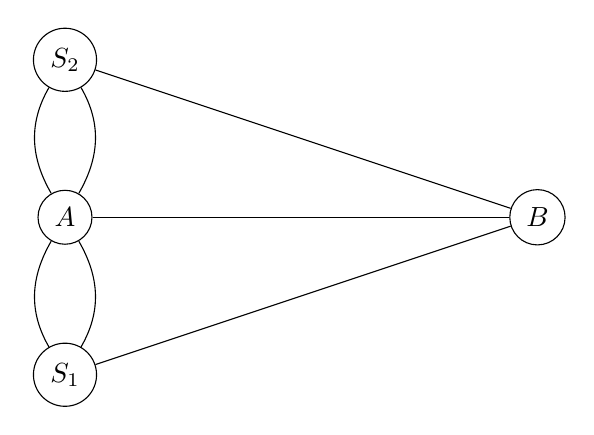
\begin{tikzpicture}
\node[draw,circle](S_1) at (0,0){$S_1$};
\node[draw,circle](S_2) at (0,4){$S_2$};
\node[draw,circle](A) at (0,2){$A$};
\node[draw,circle](B) at (6,2){$B$};
\draw (S_1) to [out=60,in=-60] (A);
\draw (S_1) to [out=120,in=-120] (A);
\draw (A) to [out=60,in=-60] (S_2);
\draw (A) to [out=120,in=-120]  (S_2);
\draw (A)--(B);
\draw (S_1)--(B);
\draw (S_2)--(B);

\end{tikzpicture}
\caption{Königsberger Brückenproblem}
\label{kb}
\end{figure}

Die Aufgabe war nun, einen Weg über die Brücken zu finden, sodass jede Brücke genau einmal überquert wurde. Da niemand eine Lösung fand, schien diese Aufgabe nicht lösbar zu sein. Im Jahre 1736 schließlich gelang es Leonhard Euler (1707--1783) zu beweisen, dass es einen solchen Weg nicht gibt. Nach ihm wurde diese Art von Wegen in der Graphentheorie \glqq Eulerweg\grqq{}  genannt.

Ein ähnliches Problem ist Mitte des neunzehnten Jahrhunderts durch ein von Sir William Rowan Hamilton (1805--1865) erfundenes Spiel namens \glqq Icosian Game\grqq{} zum Thema Reiserouten entstanden, wodurch diese Art von Problemen als \glqq Hamiltonweg\grqq{} bezeichnet wird.

\subsection{Eulerweg und -kreis}
\label{sec.Euler}


Ein \wichtig{Eulerweg} ist ein Weg, der \wichtig{alle Kanten} eines Graphen genau einmal abläuft. Eulerwege sind zum Beispiel bei einer Stadtbesichtigung interessant, wenn wir uns nicht für bestimmte Kreuzungen oder Stationen interessieren, sondern für die verschiedenen Straßen. Kurz gesagt besuchen wir jede Straße genau einmal.

Ein \wichtig{Eulerkreis} ist ein spezieller Eulerweg. Dieser endet im gleichen Knoten, in dem er auch beginnt.

Besitzt ein Graph G einen Eulerkreis, wird er \wichtig{eulersch} genannt.


\begin {fakt}
Ein Graph G besitzt genau dann einen Eulerweg, wenn maximal zwei Knoten einen ungeraden Grad haben.
\end{fakt}

\begin {proof}
Wenn wir über eine Kante an einem Knoten ankommen, müssen wir ihn über eine andere Kante wieder verlassen. Dadurch fallen bei jedem Besuch eines Knotens exakt zwei mögliche Kanten weg, über die wir den Knoten erreichen oder verlassen können. Wenn am Ende des Durchlaufens aller Knoten alle Kanten abgelaufen sein sollen, müssen alle Knoten eine gerade Anzahl von Kanten besitzen, die von ihm ausgehen -- mit Ausnahme des Anfangs- und Endknotens. Der Knoten, an dem wir den Eulerweg beginnen, muss einmal mehr verlassen als betreten werden, während der Endknoten einmal mehr angelaufen als verlassen wird. Daher dürfen diese beiden Knoten einen ungeraden Grad besitzen, während die restlichen Knoten einen geraden Grad haben.
\end {proof}

\begin {fakt}
\label{EKreis}
Ein Graph G besitzt genau dann einen Eulerkreis, wenn \wichtig{alle} Knoten einen geraden Grad haben.
\end {fakt}

\begin {proof}
Um die Äquivalenz zu beweisen, erklären wir erst die eine Schlussfolgerungsrichtung und anschließend die andere.

Genau wie beim Eulerweg folgt aus der Euler-Eigenschaft, dass wir gerade Grade brauchen. Da wir in diesem Fall allerdings am Startknoten wieder ankommen müssen, müssen diesmal \textit{\wichtig{alle}} Knoten einen geraden Grad haben. Sonst landen wir an einem Knoten, den wir nicht wieder verlassen können, und können keinen Kreis schließen.

Anders herum soll aus einem Graphen, welcher nur gerade Grade besitzt, folgen, dass ein Eulerkreis existiert.
Wenn wir am Startknoten wieder ankommen, ohne vorher alle Kanten abgelaufen zu haben, markieren wir die abgelaufenen Kanten und suchen uns einen Knoten, welcher sowohl abgelaufene als auch noch nicht besuchte Kanten besitzt. Von dort laufen wir wieder über alle noch nicht markierten Kanten, bis wir an demselben Knoten wieder ankommen und wiederholen diesen Vorgang so lange, bis der ganze Graph abgelaufen ist. Die jeweiligen Startknoten sind die Verbindungsstellen der kleineren Eulerkreise, über welche wir diese zu einem großen Eulerkreis verbinden können.
\end {proof}

\subsection{Hamiltonweg und -kreis}

Bei \wichtig{Hamiltonwegen} läuft man nicht wie in Abschnitt \ref{sec.Euler} alle \wichtig{Kanten} ab, sondern alle \wichtig{Knoten}. Jeder Knoten wird genau einmal besucht, aber es muss nicht jede Kante abgelaufen werden.

Analog zum Eulerkreis ist der \wichtig{Hamiltonkreis} ein spezieller Hamiltonweg, bei welchem der Start- gleich dem Endknoten ist.

Besitzt ein Graph G einen Hamiltonkreis, wird er \wichtig{hamiltonsch} genannt.

\subsection{Der Petersen-Graph}

Ein besonderer Graph ist der Petersen-Graph, den wir im Folgenden im Zusammenhang mit Euler- sowie Hamiltonkreisen untersuchen werden. Er besitzt 10 Knoten und 15 Kanten, wobei alle Knoten Grad drei besitzen.
Weiterhin können wir ihn in einen äußeren (Fünfeck) und einen inneren Bereich (Stern) unterteilen, welche durch fünf Kanten verbunden sind.

\begin{figure}[ht]
\centering
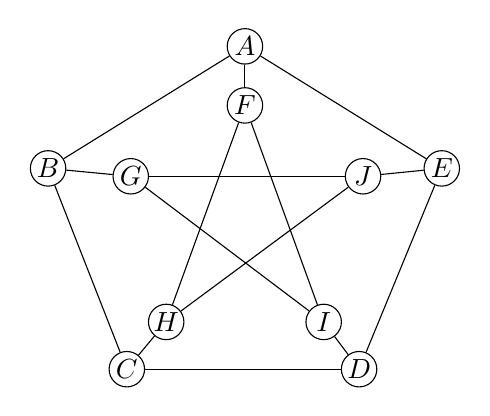
\begin{tikzpicture}

\node[minimum width=0.45cm,draw,circle](1)at(-2.5,-0.5){};
\node[minimum width=0.45cm,draw,circle](2)at(0,-2.05){};
\node[minimum width=0.45cm,draw,circle](3)at(-1.05,-4.6){};
\node[minimum width=0.45cm,draw,circle](4)at(-4,-4.6){};
\node[minimum width=0.45cm,draw,circle](5)at(-5,-2.05){};
\node[minimum width=0.45cm,draw,circle](6)at(-2.5,-1.25){};
\node[minimum width=0.45cm,draw,circle](7)at(-1,-2.15){};
\node[minimum width=0.45cm,draw,circle](8)at(-1.5,-4){};
\node[minimum width=0.45cm,draw,circle](9)at(-3.5,-4){};
\node[minimum width=0.45cm,draw,circle](10)at(-3.95,-2.15){};

\node(11)at(-2.5,-0.5){$A$};
\node(21)at(0,-2.05){$E$};
\node(31)at(-1.05,-4.6){$D$};
\node(41)at(-4,-4.6){$C$};
\node(51)at(-5,-2.05){$B$};
\node(61)at(-2.5,-1.25){$F$};
\node(71)at(-1,-2.15){$J$};
\node(81)at(-1.5,-4){$I$};
\node(91)at(-3.5,-4){$H$};
\node(101)at(-3.95,-2.15){$G$};

\draw(1)--(2);
\draw(2)--(3);
\draw(3)--(4);
\draw(4)--(5);
\draw(1)--(5);
\draw(1)--(6);
\draw(2)--(7);
\draw(3)--(8);
\draw(4)--(9);
\draw(10)--(5);
\draw(6)--(8);
\draw(6)--(9);
\draw(7)--(9);
\draw(7)--(10);
\draw(8)--(10);

\end{tikzpicture}
\caption{Der Petersen-Graph.}
\label{fig:wiki}
\end{figure}

Wenn wir die Grade der Knoten betrachten, können wir schnell feststellen, dass im Petersengraph kein Eulerweg existiert, da mehr als zwei Knoten, nämlich alle zehn, einen ungeraden Grad besitzen.

\wichtig{Existiert ein Hamiltonkreis?}
Graphentheoretisch sind der innere und der äußere Teil des Graphen gleich, miteinander verbunden besitzen sie jedoch gegensätzliche Arten von Symmetrie: den äußeren Teil könnte man einfach im oder gegen den Uhrzeigersinn ablaufen, im Inneren erreicht man jedoch immer jeden zweiten Knoten, wenn man die Knoten entsprechend der Darstellung im Uhrzeigersinn abläuft. Beim Hamiltonkreis muss der Weg mit demselben Knoten enden, mit dem er auch begonnen hat, und deshalb entweder zweimal oder viermal zwischen dem Inneren und dem Äußeren wechseln.

Im Falle, dass man einmal vom äußeren zum inneren und einmal vom inneren zum äußeren Kreis wechselt, müsste man den jeweiligen Kreis vor dem Wechsel komplett ablaufen. Im inneren Kreis würde man beim Ablaufen des inneren Teilweges an einem anderen Knoten ankommen, als wenn man den Außenkreis abläuft. So können wir den Innenkreis nicht an dem Knoten beenden, der mit dem Anfangsknoten des Außenkreises verbunden ist. Es kann also kein Hamiltonkreis geschlossen werden.

Im Fall von vierfachem Kreiswechsel wird genau eine der Verbindungen zwischen Innen- und Außenkreis nicht abgelaufen. Dies sei o.\,B.\,d.\,A. $\{A,F\}$. Wenn $\{A,F\}$ nicht abgelaufen wird, muss A mit B und E verbunden werden. Da außer $\{A,F\}$ alle Verbindungen zwischen Innen- und Außenkreis abgelaufen werden müssen, ist ein Teilstück des Weges nun G-B-A-E-J. Von J und G gibt es nun abgesehen von $\{G,J\}$, die an dieser Stelle eingebaut den Kreis beenden würde, nur noch die Verbindungen zu I und H. Unser bisheriger Weg wäre also I-G-B-A-E-J-H. Von I und H aus müssen wir nun wegen des vierfachen Kreiswechsels wieder in den Außenkreis zu C bzw. D wechseln, wodurch der Kreis zwar geschlossen wird, F jedoch kein Teil dieses Kreises ist.

Somit existiert im Petersengraph kein Hamilton\wichtig{kreis}.
